\chapter{Einführung}

\section{Motivation}

Die Entwicklung und Verbesserung von Frameworks zur Verarbeitung großer Datenmengen ist zur Zeit hochaktuell und zunehmend im Fokus von Medien und Unternehmen. Verschiedene Programme und Paradigmen konkurrieren um die schnellste, bequemste und stabilste Art großen Datenmengen einen geschäftsfördenden Nutzen abzuringen.\\

Mit dem Begriff "`große Datenmengen"' oder "`Big Data"' werden in dieser Arbeit solche Datenmengen zusammengefasst, die die Kriterien Volume, Velocity, Variety \footcite{Lan01} erfüllen oder "`Datenmengen, die nicht mehr unter Auflage bestimmter \gls{sla}s auf einzelnen Maschinen verarbeitet werden können"' (Vgl. \cite{Sam14}).\\

Als Unternehmen, das früh mit solchen Datenmengen konfrontiert war implementierte Google das Map-Reduce Paradigma \footcite{Dean04} als Framework zur Ausnutzung vieler kostengünstiger Rechner für verschiedene Aufgaben (u.a.  Indizierung von Webseiten und PageRank \footcite{page2001method}). \\

In Folge der Veröffentlichung dieser Idee im Jahr 2004 wurde Map-Reduce in Form der OpenSource Implementation Hadoop (gemeinsam mit einer Implementation des Google File Systems GFS, u.a.) \footcite{Ghema03} zum de-facto Standard für Big-Data-Analyseaufgaben.\\

Reines Map-Reduce (nach Art von Hadoop) als Programmierparadigma zur Verarbeitung großer Datenmengen zeigt jedoch in vielen Anwendungsfällen Schwächen:
\begin{itemize}
	\item Daten, die in hoher Frequenz entstehen und schnell verarbeitet werden sollen erfordern häufiges Neustarten von Map-Reduce-Jobs. Die Folge ist kostspieliger Overhead durch Verwaltung/Scheduling der Jobs und gegebenenfalls wiederholtem Einlesen von Daten.
	\item Algorithmen die während ihrer Ausführung iterativ Zwischenergebnisse erzeugen und auf vorherige angewiesen sind (häufig bei Maschinenlernalgorithmen) können nur durch persistentes Speichern der Daten und wiederholtes Einlesen zwischen allen Iterationsschritten implementiert werden.
	\item Anfragen an ein solches Map-Reduce-System erfolgen imperativ in Form von kleinen Programmen. Dieses Verfahren ist offensichtlich nicht so intuitiv und leicht erlernbar wie deklarative Abfragesprachen klassischer Datenbanken (z.B. SQL).
\end{itemize}

In der Folge dieser Probleme entstanden viele Ansätze dieses Paradigma zu ersetzen, zu ergänzen oder durch übergeordnete Ebenen und High-Level-APIs zu vereinfachen \footcite{Sin14}.\\

Eine der Alternativen zu der Map-Reduce-Komponente in Hadoop ist die "`general engine for large-scale data processing"' Apache Spark.\\

Ein Indiz für das steigende Interesse an diesem Produkt liefert unter anderem ein Vergleich des Interesses an Hadoop und Spark auf Google:\\

\begin{figure}[h]
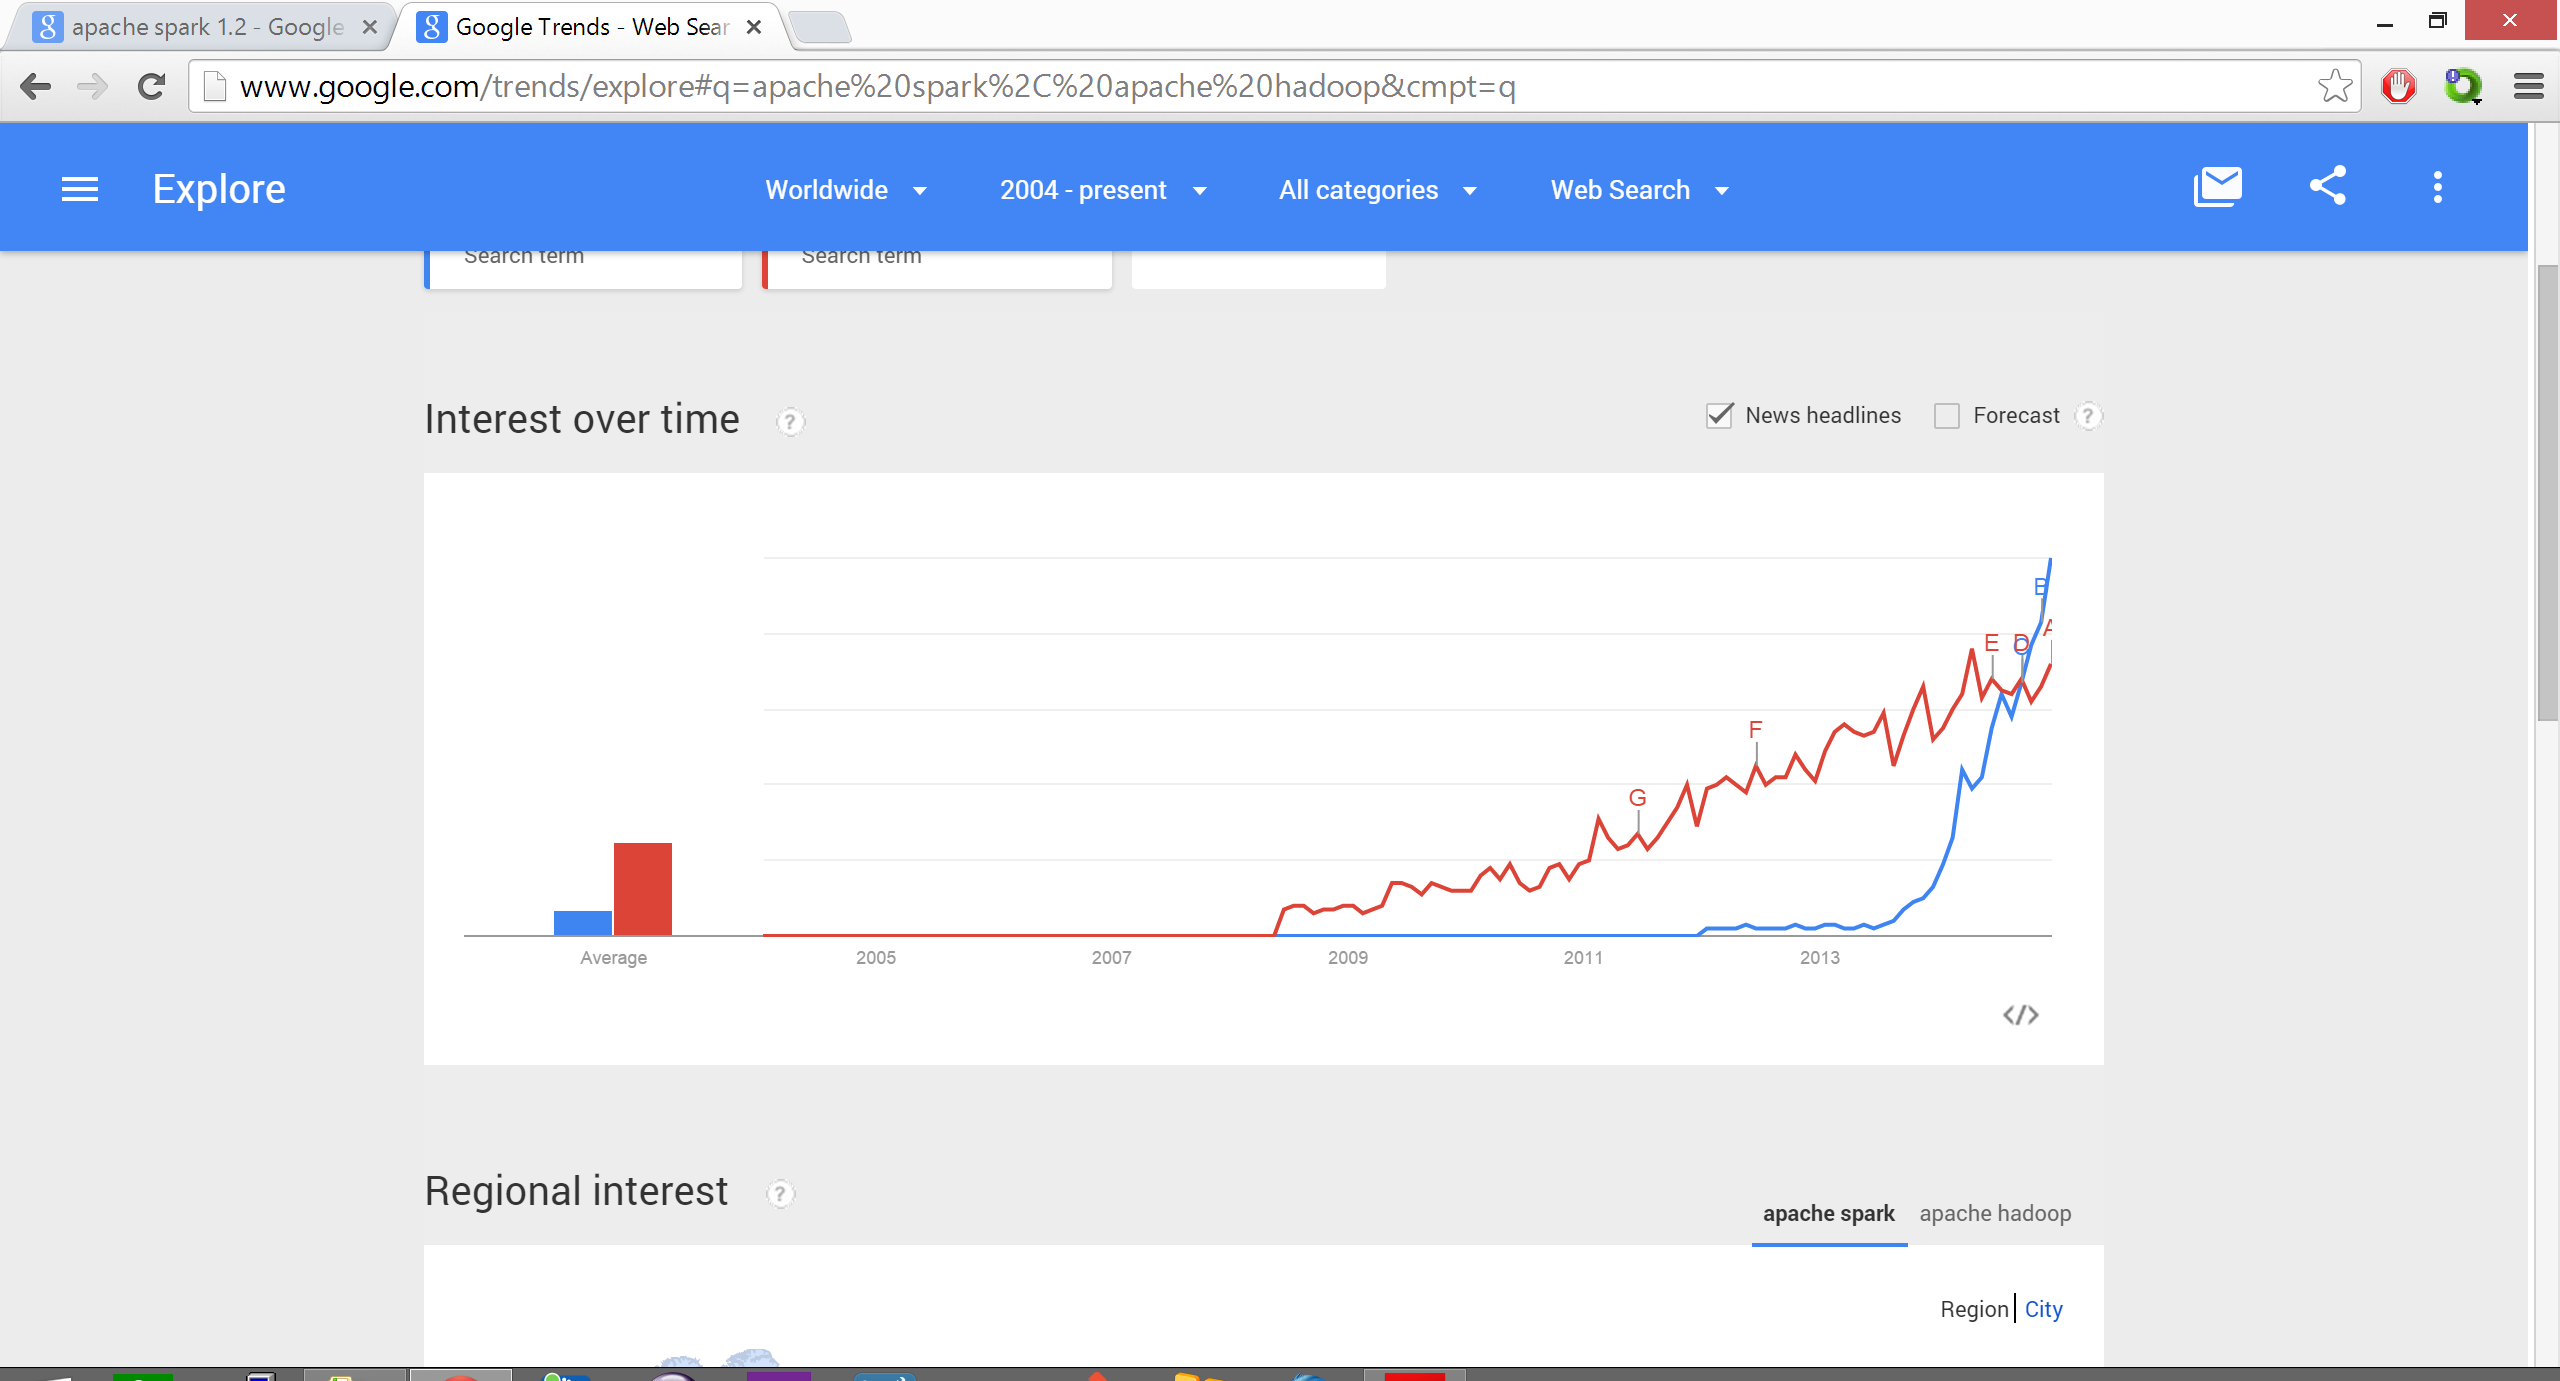
\includegraphics[scale=0.6]{bilder/trends_spark_vs_hadoop.PNG}
\caption[Google Trends]{Vergleich der Suchanfragen zu Spark und Hadoop, Stand 24.03.2014 \cite{googletrends}}
\end{figure}

\section{Kontextabgrenzung}
Das Ziel dieser Arbeit ist es eine Analyse und Bewertung der grundlegenden Konzepte und Anwendungsmöglichkeiten von Apache Spark zu vermitteln.

Für ein tieferes Verständnis werden Installation, Cluster-Betrieb und die Modellierung und Implementation von Treiberprogrammen beispielhaft durchgeführt, dokumentiert und bewertet. Hierbei kommt Apache Spark in der Version 1.3.0 zum Einsatz.\\

Nur am Rande wird betrachtet:
\begin{itemize}
	\item Der Vergleich mit ähnlichen Produkten
	\item Die Empirische Messung des Skalierungsverhaltens
	\item Details zu Installation und Betrieb
\end{itemize}
